\documentclass[bigger]{beamer}

\usepackage{booktabs}
\useinnertheme{rounded}
\usecolortheme{crane}
\setbeamerfont{block title}{size={}}

\title{Should We Give Learners Control Over Item Difficulty?}

\author{Jan Papou\v{s}ek and \textbf{Radek Pel\'anek}\\[10mm]
%Masaryk University Brno\\
%Czech Republic

\includegraphics[width=.3\linewidth]{al-logo}
}

\date{PALE 2017}
 
\begin{document}

\frame{\titlepage}

\begin{frame}
  \frametitle{outlinemaps.org}
	\noindent\makebox[\textwidth]{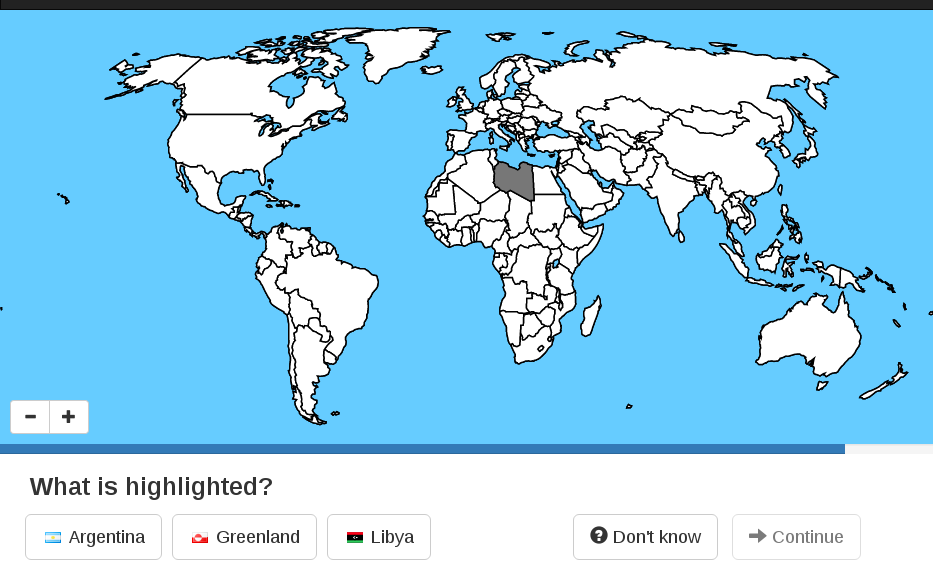
\includegraphics[width=\paperwidth]{slepemapy_world_practice}}
\end{frame}

\begin{frame}
  \frametitle{outlinemaps.org}
	\noindent\makebox[\textwidth]{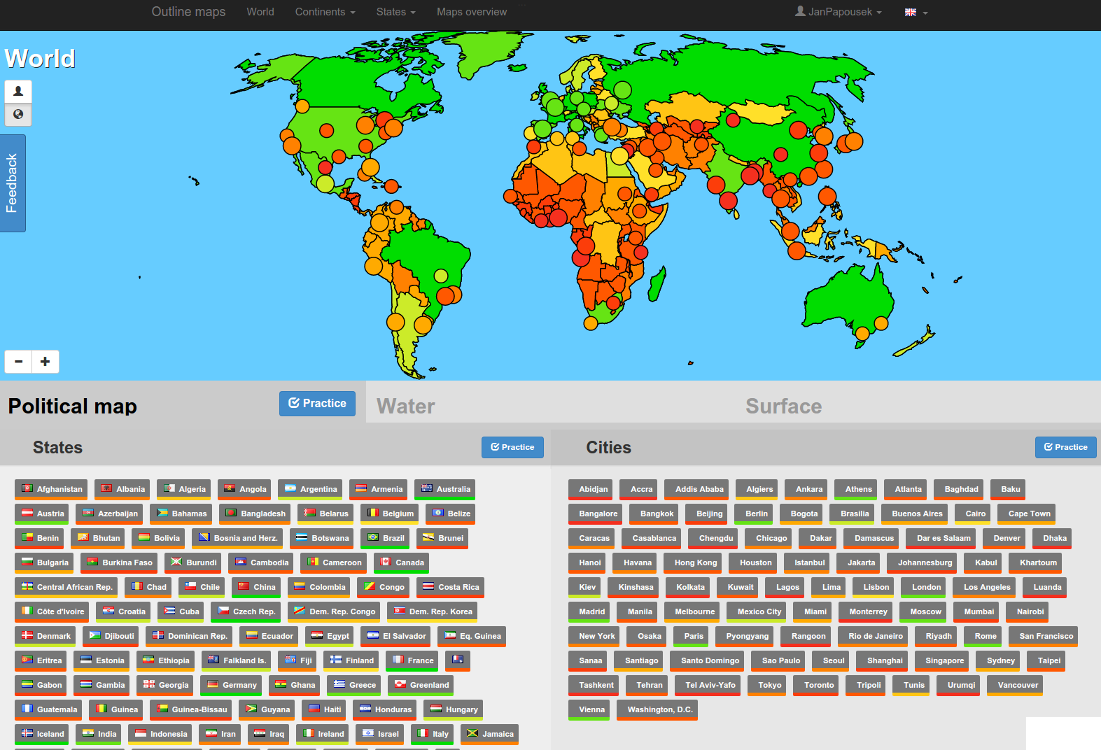
\includegraphics[width=\paperwidth]{slepemapy_world}}
\end{frame}

\begin{frame}
  \frametitle{Questions of Suitable Difficulty}

  \begin{itemize}
  \item data on performance $\Rightarrow$ learner modeling $\Rightarrow$
    estimate of knowledge
  \item estimate of knowledge $\Rightarrow$ choice of suitable question
  \item target difficulty of questions
    \begin{itemize}
    \item previous experiment
    \item best results for 35\% error rate
    \end{itemize}
  \end{itemize}
\end{frame}

\begin{frame}
  \frametitle{Idea}

  \begin{block}{}
    Give learners control over target difficulty.
  \end{block}

  \begin{itemize}
  \item research question: is it beneficial?
  \item specific version of more general problem: giving users control vs
    automatic decisions
  \item closely relevant previous experiment: Math Garden, this experiment much
    larger (millions of answers)
  \end{itemize}
\end{frame}

\begin{frame}
  \frametitle{Realization}

  practice divided into series of 10 questions

  \bigskip

  \begin{center}
    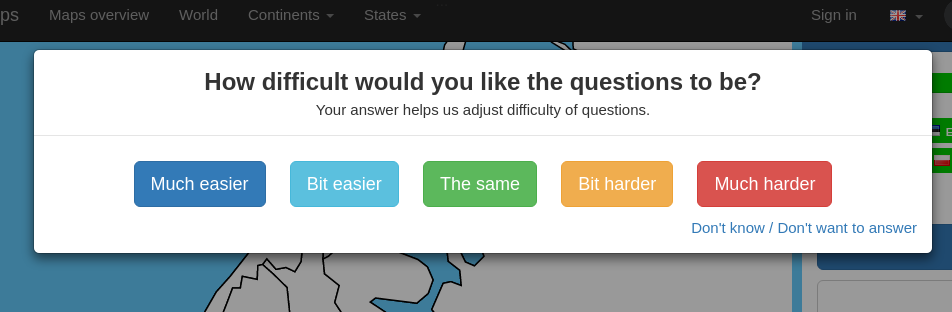
\includegraphics[width=\linewidth]{modal}
  \end{center}
\end{frame}

\begin{frame}
  \frametitle{Experimental Conditions}

  \begin{center}
    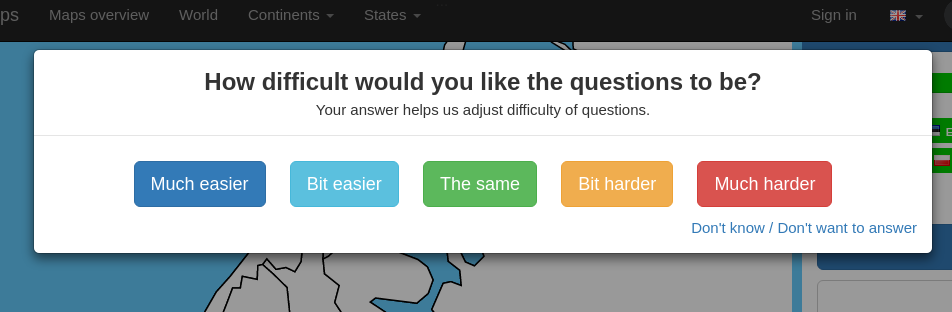
\includegraphics[width=.65\linewidth]{modal}
  \end{center}

  \medskip

  \begin{itemize}
  \item \textbf{normal} -- no dialog box
  \item \textbf{placebo} -- dialog box, without effect
  \item \textbf{adjustment} -- dialog box with effect
  \end{itemize}
\end{frame}

\begin{frame}
  \frametitle{Ratings}

  \begin{center}
    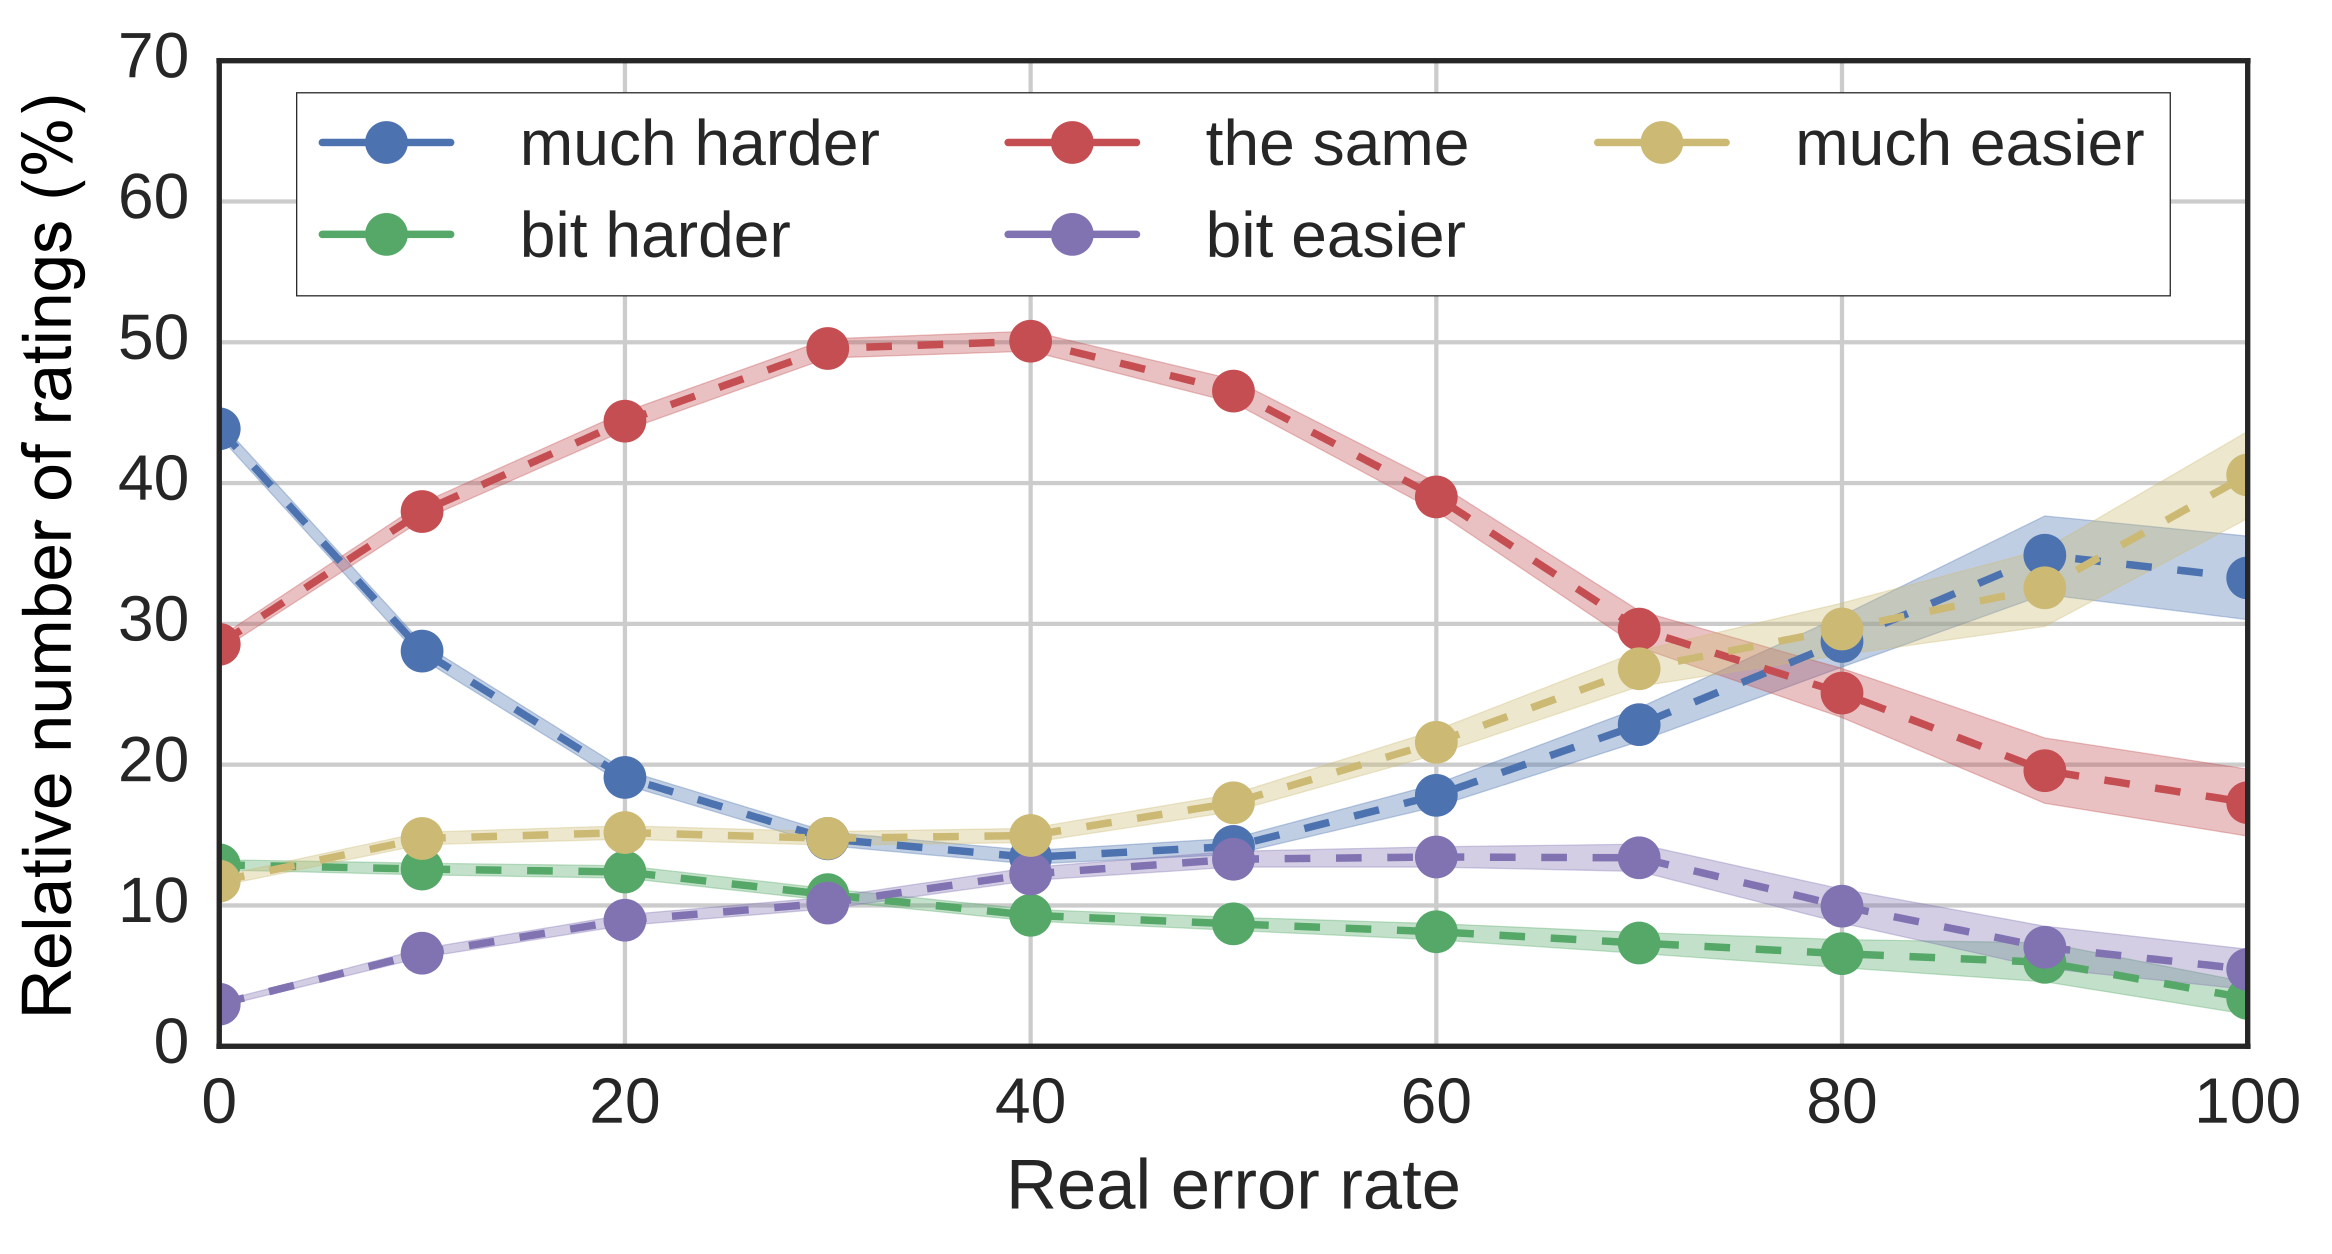
\includegraphics[width=\linewidth]{ratings}
  \end{center}
\end{frame}

\begin{frame}
  \frametitle{Engagement and Learning}

  overall results: small differences among conditions

  \medskip

  \begin{itemize}
  \item engagement: dialog box reduces engagement, adjustment not sufficient to
    overweight this disadvantage
  \item learning: no significant differences
  \end{itemize}
\end{frame}

\begin{frame}
  \frametitle{Disaggregated Results}

  \begin{center}
    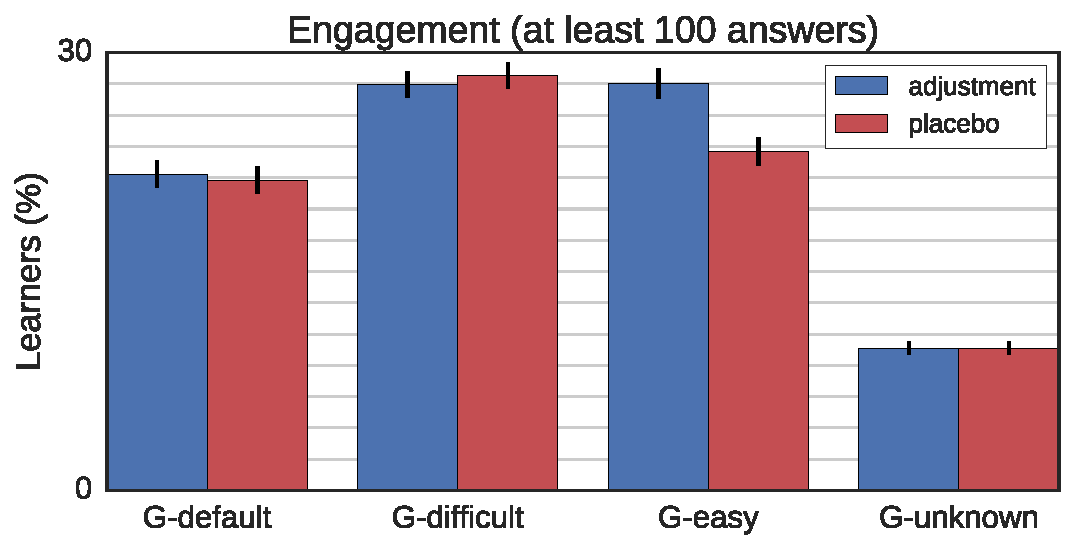
\includegraphics[width=.6\linewidth]{survival_by_ratings}

    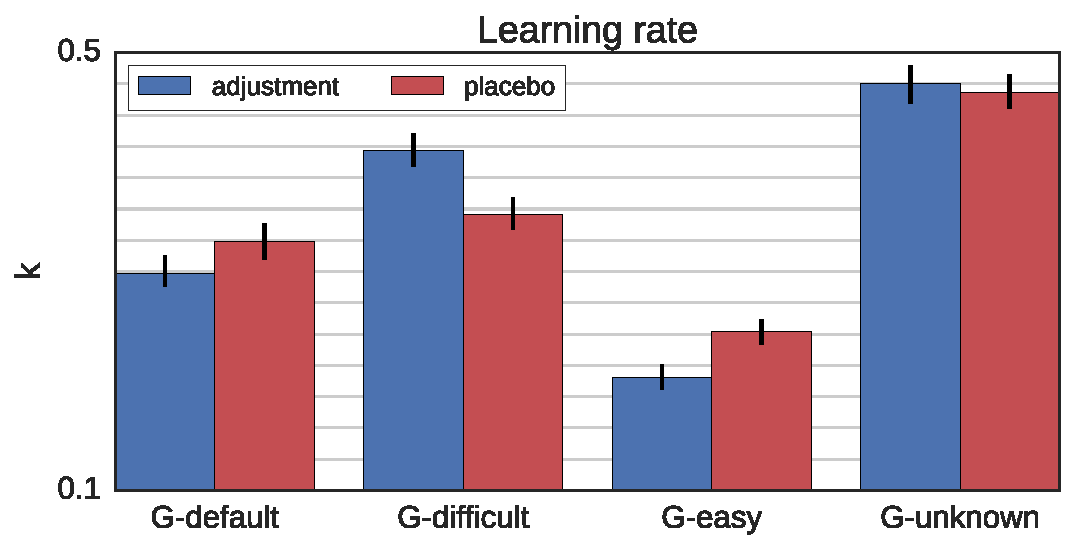
\includegraphics[width=.6\linewidth]{learning_by_ratings_slope}
  \end{center}
\end{frame}

\begin{frame}
  \frametitle{Summary}

  \begin{itemize}
  \item overall: giving learners control over question difficulty not beneficial
  \item warning for similar research: presence of irony in learners' responses
  \end{itemize}
\end{frame}

\begin{frame}
  \frametitle{Issues for Discussion}

  \begin{itemize}
  \item circumstances under which it is beneficial to give users control over
    settings
  \item specific hypotheses for experiments
  \item irony in user responses
  \end{itemize}
\end{frame}

\end{document}